\documentclass[11pt]{article}

\usepackage[margin=0.9in]{geometry}
\usepackage{array}
\usepackage{booktabs}
\usepackage{enumitem}
\usepackage{hyperref}
\usepackage{longtable}
\usepackage{tikz}
\usepackage{xcolor}
\usepackage{amsmath}
\usepackage{url}

\usetikzlibrary{arrows.meta,positioning,shapes.geometric}

\hypersetup{
  colorlinks=true,
  linkcolor=blue!45!black,
  urlcolor=blue!45!black
}

\setlist[itemize]{leftmargin=*, itemsep=2pt, topsep=3pt}
\setlist[enumerate]{leftmargin=*, itemsep=2pt, topsep=3pt}
\renewcommand{\arraystretch}{1.15}

\newcommand{\code}[1]{\path{#1}}
\newcommand{\state}[1]{\textsf{#1}}
\newcommand{\action}[1]{\texttt{#1}}
\newcommand{\roundid}[1]{\texttt{round #1}}

\title{\vspace{-0.3in}Multi-Turn Policy Learning for Table-Fill Aggregation}
\author{Internal technical white paper}
\date{July 2026}

\begin{document}
\maketitle

\begin{abstract}
The table-fill pipeline has evolved from a single question-answering pass into
an iterative aggregation system.  Each outer round decides which parts of the
answer universe remain unknown, searches for candidate sources, ingests any
accepted sources into the knowledge graph, materializes answer-view tables,
recovers best-guess sidecar fields, scores marginal table progress, and plans
the next frontier.  The current implementation is stateful: it records source
acceptance, duplicate and blocked URLs, failed operators, completion issues,
best-guess operator yields, and table-level reward.  It is not yet a learned
controller.  Most routing decisions still come from finite operator orders and
single-call prompt judgments.

This document specifies the current control loop, shows how strategy is
adapting today using the latest round-27b trace, identifies the missing
decision-state abstraction, and proposes a staged multi-turn reinforcement
learning design.  The proposed design keeps the existing generic table-fill
machinery, adds durable state--action--observation--reward trajectory records,
wraps current heuristic routing in a policy interface, and introduces offline
policy evaluation before any online exploration.
\end{abstract}

\section{Purpose and Scope}

The system is trying to solve a data aggregation task, not merely produce a
natural-language answer.  Given one or more table specifications and a question,
it should grow evidence-backed tables until the task-level completion criteria
are defensible.  A full iteration of that process is an \emph{outer round}.  One
outer round can include many catalog searches, many deficit searches, several
source ingestions, one or more GASL executions, table export, best-guess
recovery, reward scoring, completion estimation, and frontier expansion.

The desired long-term behavior is adaptive in the reinforcement-learning sense:
the agent should learn which strategy works for a class of current states,
observe what it spent and what it gained, and improve future choices.  The
current implementation has the right event surfaces for that, but it does not
yet store trajectories in a form that a learner can consume.

\subsection{Repository context}

The current table-fill loop is centered in the following modules:

\begin{itemize}
  \item \code{question_pipeline/pipeline.py}: orchestration, outer rounds,
  Firecrawl harvesting, graph ingestion, GASL, table exports, completion
  updates, and frontier expansion.
  \item \code{question_pipeline/goals.py}: table profiles, count deficits, row
  gap deficits, and task-level stop-state construction.
  \item \code{question_pipeline/completion.py}: persistent completion scope,
  open bins, open estimate issues, and actionability checks.
  \item \code{question_pipeline/search.py}: durable search tasks, frontier
  scheduling, candidate acceptance, and harvest outcomes.
  \item \code{question_pipeline/search_memory.py}: cross-round aggregation of
  successful and failed target-search attempts.
  \item \code{question_pipeline/strategy.py}: LLM query construction for
  catalog and target deficits.
  \item \code{question_pipeline/strategy_state.py}: deterministic operator
  routing, failure classification, and operator exhaustion.
  \item \code{question_pipeline/progress_judge.py}: generic source-progress
  relevance judgments.
  \item \code{question_pipeline/best_guess.py}: deterministic and LLM
  best-guess sidecar recovery operators.
  \item \code{question_pipeline/reward.py}: marginal reward for table growth,
  provenance, sidecar recovery, and duplicate/source-repeat penalties.
\end{itemize}

\section{Current Control Loop}

\subsection{Outer-round definition}

The table-fill \emph{round} must mean the largest iterative loop in the
pipeline.  In the current code that loop is \code{QuestionPipeline.run()}.
Smaller operations such as a search wave, a best-guess operator, or a GASL
iteration are sub-actions inside one outer round.

At a high level, an outer round performs the following steps:

\begin{enumerate}
  \item Drain pending search tasks from the \code{SearchFrontier}.
  \item Harvest search results, scrape accepted pages, and record one
  \code{SearchOutcome} per search task.
  \item Ingest accepted papers into the current graph.
  \item Select a source-local graph for GASL and seed source nodes.
  \item Execute GASL against the declared answer-view tables.
  \item Export declared tables and derived artifacts.
  \item Recover best-guess sidecar fields from existing row, source, chunk, and
  KG context.
  \item Score marginal table progress against the previous snapshot.
  \item Estimate completion, critique the estimate, and persist open bins.
  \item Build fill deficits and enqueue the next search frontier.
\end{enumerate}

Rounds with no newly accepted paper still write carried-forward tables, refresh
completion and search memory, and enqueue more frontier work when the goal is
not complete.  This is important because a zero-source round still changes the
policy state: it distinguishes ``we have not tried this'' from ``this operator
on this deficit produced no hits, duplicates, or irrelevant pages.''

\begin{figure}[htbp]
\centering
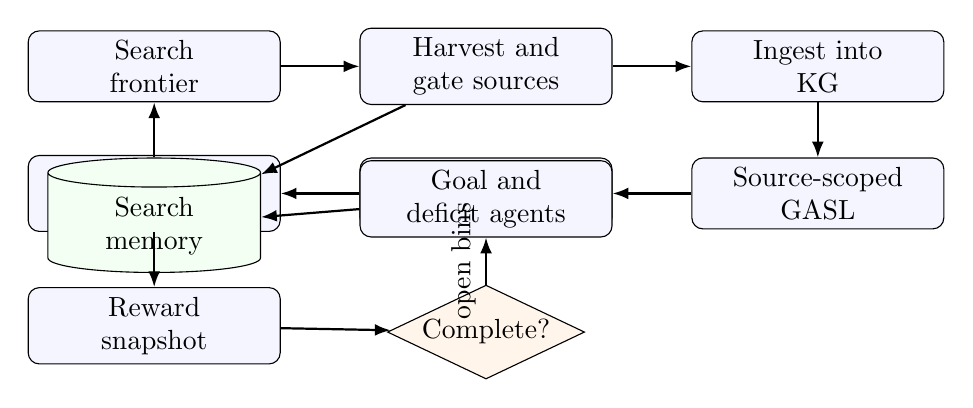
\begin{tikzpicture}[
  node distance=7mm and 10mm,
  box/.style={draw, rounded corners, align=center, minimum width=32mm,
    minimum height=9mm, fill=blue!4},
  store/.style={draw, cylinder, shape border rotate=90, aspect=0.25,
    align=center, minimum width=27mm, minimum height=11mm, fill=green!5},
  decision/.style={draw, diamond, aspect=2.1, align=center, inner sep=1pt,
    fill=orange!8},
  arr/.style={-{Latex[length=2mm]}, thick}
]
\node[box] (frontier) {Search\\frontier};
\node[box, right=of frontier] (harvest) {Harvest and\\gate sources};
\node[box, right=of harvest] (ingest) {Ingest into\\KG};
\node[box, below=of ingest] (gasl) {Source-scoped\\GASL};
\node[box, left=of gasl] (tables) {Answer-view\\tables};
\node[box, left=of tables] (guess) {Best-guess\\recovery};
\node[box, below=of guess] (reward) {Reward\\snapshot};
\node[decision, below=of tables] (complete) {Complete?};
\node[box, below=of harvest] (deficit) {Goal and\\deficit agents};
\node[store, below=of frontier] (memory) {Search\\memory};

\draw[arr] (frontier) -- (harvest);
\draw[arr] (harvest) -- (ingest);
\draw[arr] (ingest) -- (gasl);
\draw[arr] (gasl) -- (tables);
\draw[arr] (tables) -- (guess);
\draw[arr] (guess) -- (reward);
\draw[arr] (reward) -- (complete);
\draw[arr] (complete) -- node[above, sloped]{open bins} (deficit);
\draw[arr] (deficit) -- (memory);
\draw[arr] (memory) -- (frontier);
\draw[arr] (harvest) -- (memory);
\end{tikzpicture}
\caption{Current table-fill feedback loop.  Search memory and completion state
make the loop stateful, but the action policy is still heuristic.}
\label{fig:current-loop}
\end{figure}

\section{How Strategy Adapts Today}

\subsection{Completion and deficit adaptation}

\code{TableFillGoalTracker} computes a compact profile of each deliverable
table: observed row counts, missing required and completeness columns, row gap
examples, candidate columns, and the currently known universe estimate.  It
then emits \code{FillDeficit} objects for two broad purposes:

\begin{itemize}
  \item \textbf{Count shortfalls}: the estimated answer universe says a table
  needs more rows or a row family remains undersampled.
  \item \textbf{Gap saturation}: the table has rows, but key columns or
  sidecar columns are sparse enough to justify targeted searches.
\end{itemize}

\code{completion.py} tracks whether the estimate of the answer universe is
actionable.  The stop criteria are tied to the task state, not a fixed number
of iterations.  An estimate is actionable only after the system has recorded
enough search-space probes, resolved blocking issues, and closed or justified
the underexplored bins.

\subsection{Target-search adaptation}

Deficit searches are stateful at two levels.  First,
\code{SearchMemory.from_outcomes()} folds prior attempts into a per-target
record containing accepted URLs, duplicate URLs, failed and successful query
terms, missing needs, off-topic axes, avoid cues, and better-search cues.
Second, \code{plan_target_operator()} classifies the latest failure and chooses
the next finite operator.

The current target operator families are generic.  They change the shape of a
query rather than the data domain:

\begin{itemize}
  \item exact anchors: preserve specific anchors when previous context looked
  promising;
  \item context pivots: move from a failed anchor to adjacent context terms;
  \item anchor drops: remove overly narrow anchors that caused duplicate or
  zero-hit searches;
  \item terminology swaps: change surface terms while preserving the slot need;
  \item source shifts: change the family of likely source rather than the slot.
\end{itemize}

This is real adaptation, but it is not learned adaptation.  The transition from
one operator to the next is encoded in \code{strategy_state.py}.  The LLM is
asked to instantiate a query under the chosen operator constraints.

\subsection{Catalog adaptation}

Catalog tasks are broader than target deficits.  They try to bound the search
space: systematic reviews, datasets, dashboards, source families, and broad
row families.  Catalog outcomes are annotated with later graph and table deltas
so the next round can tell whether a broad source family produced material
progress.

\subsection{Source relevance adaptation}

When \code{--source-relevance-mode focused} is enabled, each candidate source is
judged by the reusable progress judge before scraping and ingestion.  The judge
receives the task goal, deficit context, compact result metadata, and a snippet
of source text.  It emits a verdict plus structured fields such as matched
needs, missing needs, better-search cues, avoid cues, and off-topic axes.  Those
fields flow into the search outcome and then into \code{SearchMemory}.

The relevance gate is a decision point with delayed reward: a source that looks
useful may fail to add graph entities or table rows, while an initially modest
source can be high-yield because its supplementary text contains dense tables.
The current code records both the immediate gate judgment and the later graph
or table delta, but it does not yet train the gate against delayed reward.

\subsection{Best-guess adaptation}

Best-guess recovery currently has state and accounting, but its operator order
is fixed.  For each missing sidecar slot, the runner tries deterministic local
operators and then LLM operators:

\begin{enumerate}
  \item \action{same\_row\_scan}
  \item \action{sibling\_row\_scan}
  \item \action{source\_metadata\_extract}
  \item \action{source\_chunk\_extract}
  \item \action{kg\_neighbor\_extract}
\end{enumerate}

The derived \action{best\_guess\_strategy\_state} artifact reports gross and
marginal accepted row slots by operator plus overlap between operators.  That
is enough to evaluate which operators produce non-overlapping yield for a
given table, but it is not yet used to reorder the next batch.

\subsection{Reward adaptation}

\code{score_table_fill_snapshot()} converts a pair of table snapshots into a
scalar marginal reward.  The current \action{table\_fill\_v2} reward makes new
source-backed field/value facts and accepted best-guess slots the primary
positive terms.  Row identities and row-slot counts remain diagnostic terms
with small weights, while duplicate identities and repeated source support
beyond a capped per-value depth target are penalized.

The reward is useful as an empirical signal, but today it is reported rather
than fed back as an optimization target.  It also lacks an explicit cost term
for Firecrawl calls, LLM calls, token volume, scrape bytes, and wall-clock time.

\section{Round-27b Case Study}

The live round-27b run exercises the current adaptive machinery on a focused
source-level table with columns for reproduction-number estimates, date or
time interval, location, strain or variant, model basis, uncertainty, and
provenance.  The durable artifacts at the sampling point contained completed
outer rounds 27--29 and search outcomes for round 30.

\begin{table}[htbp]
\centering
\small
\begin{tabular}{@{}p{0.09\linewidth}p{0.22\linewidth}p{0.12\linewidth}p{0.10\linewidth}p{0.12\linewidth}p{0.25\linewidth}@{}}
\toprule
Round & Operators & Search outcomes & Accepted sources & Table delta & Interpretation \\
\midrule
27 &
\action{catalog\_broad\_review}, \action{target\_batch\_family},
\action{target\_exact\_anchor} &
17 & 0 & 0 rows &
The seed frontier mostly found duplicate or unusable paths; exact anchors were
too narrow for the current deficits. \\
28 &
\action{catalog\_source\_shift}, \action{target\_context\_pivot} &
20 & 1 & 999 new row identities; 40 best-guess slots &
A failed target branch pivoted away from exact anchors and accepted a dense
B.1.1.7 source, producing the only high-yield graph expansion in the sampled
trace. \\
29 &
\action{catalog\_source\_shift}, \action{target\_anchor\_drop} &
20 & 0 & 0 new rows; 6 new best-guess slots &
Anchor dropping avoided one local failure mode but did not find a new source
family.  Residual reward came only from reprocessing existing chunks. \\
30 &
\action{catalog\_terminology\_swap}, \action{target\_terminology\_swap} &
20 & 0 & no completed round record at sampling &
Term changes found a few hits but no accepted source; one hit was a known
duplicate and most target queries had zero hits. \\
\bottomrule
\end{tabular}
\caption{Sampled round-27b search behavior.  One adaptive pivot worked; later
operator changes changed syntax more than strategy.}
\label{tab:round27b}
\end{table}

\subsection{A useful pivot}

Round 27 spent five \action{target\_exact\_anchor} attempts and did not accept
a source.  The next target-search plan classified those attempts as exhausted
for that deficit and moved to \action{target\_context\_pivot}.  In round 28,
the query for a B.1.1.7 effective reproduction-number estimate in England
accepted one Science source.  After ingestion and GASL, the exported table grew
from 30 row identities to 1029 row identities.  The reward snapshot attributed
the round-28 gain to:

\begin{itemize}
  \item 999 new row identities;
  \item 19,578 newly filled row slots;
  \item 9,226 new unique cell values;
  \item 159 new distinct source IDs represented in tables;
  \item 40 new best-guess sidecar slots.
\end{itemize}

This is the desired feedback pattern.  A target-search branch failed, the
operator changed, the source gate accepted a new source, and the delayed table
reward confirmed that the branch produced useful state.

\subsection{A weak pivot}

Round 29 tried \action{target\_anchor\_drop}; round 30 tried
\action{target\_terminology\_swap}.  In the sampled trace those 20 round-30
tasks yielded seven total search hits, no accepted source, five duplicate URLs,
one Firecrawl timeout, and several zero-hit target searches.  The prompts did
change terminology and sometimes dropped a concrete anchor, but the policy did
not learn that the current target was already saturated or that broad
terminology probes were less promising than a new source family.

This is the core gap: the code observed enough data to know that one local
route had stopped paying off, but the next action was still selected by a
finite operator order rather than by expected marginal reward.

\subsection{Best-guess sidecars}

Round 28 evaluated 512 sidecar row slots.  The deterministic same-row and
sibling-row scans accepted no candidates.  LLM source metadata extraction
accepted 18 row slots, source chunk extraction accepted 19, and KG-neighbor
extraction accepted 3.  Round 29 re-evaluated the same 512-slot budget and
increased the resolved total from 40 to 43.

The state artifact already reports operator yield and overlap:

\begin{itemize}
  \item deterministic row-local operators had zero marginal yield;
  \item source metadata and chunk operators produced disjoint accepted slots;
  \item KG-neighbor extraction produced a smaller but still non-overlapping
  marginal gain;
  \item 469 of 512 row slots remained open after round 29.
\end{itemize}

This is a natural contextual-bandit surface.  The next batch should be able to
prioritize a source-local LLM extraction for row-slot types where deterministic
scans have repeatedly failed, while still preserving cheap deterministic scans
when they work on another table.

\subsection{Completion critic}

The completion state remained open after the high-yield round.  The critic kept
blocking acceptance because the run still lacked a defensible lower-bound
estimate of the answer universe, a deduplicated source-level row count, and a
granularity decision for time-series sources.  That is the correct stop-rule
behavior: a large row delta is not the same as task completion.

\section{Outcomes and Interpretation}

Table~\ref{tab:gap-analysis} separates observed outcomes from interpretation
and marks whether each outcome is in scope for the tested mechanism.

\begin{longtable}{@{}p{0.19\linewidth}p{0.28\linewidth}p{0.11\linewidth}p{0.32\linewidth}@{}}
\caption{Current adaptive behavior versus the intended mechanism.}
\label{tab:gap-analysis}\\
\toprule
Outcome & What it means & Scope & Interpretation \\
\midrule
\endfirsthead
\toprule
Outcome & What it means & Scope & Interpretation \\
\midrule
\endhead
\bottomrule
\endfoot
Round 28 accepted one source after moving from exact anchors to a context
pivot. &
Failure classification and operator exhaustion can move a deficit branch away
from an unproductive local query form. &
In scope &
The current state machine can exploit short-horizon feedback when the next
finite operator is appropriate. \\
\addlinespace
Round 29 and round 30 changed operators but found no new accepted sources. &
The route changed syntax, but not necessarily expected value.  The system did
not decide to abandon, split, or reframe the deficit based on prior low yield. &
In scope &
Operator order is a hand-coded prior, not a learned value function.  Search
memory is prompt context, not a policy. \\
\addlinespace
The source relevance judge recorded better-search and avoid cues. &
The acceptance prompt emits information that can be used as policy feedback. &
In scope &
Those fields should become structured observations connected to the action
that caused them and to delayed graph and table reward. \\
\addlinespace
Best-guess source metadata and chunk extraction had all marginal sidecar yield
in the sampled rounds. &
The derived best-guess artifacts can distinguish productive operators from
unproductive ones for a specific state. &
In scope &
The next version should choose best-guess operators by expected marginal slot
resolution per cost, not by a fixed cascade. \\
\addlinespace
The round-28 table delta contained 999 new row identities from one accepted
source. &
One dense source can dominate many sparse searches. &
In scope &
Source-family and source-density prediction are critical.  Search policy
should learn to seek high-density supplementary or tabular sources when the
table needs source-level aggregation. \\
\addlinespace
The completion critic rejected round 28 and round 29 despite nonzero reward. &
Marginal table reward and task completion are different signals. &
In scope &
The reward function should be multi-objective: immediate table growth,
coverage of declared axes, lower-bound confidence, and deduplicated
source-level completeness. \\
\addlinespace
Firecrawl returned duplicate, zero-hit, blocked, and timeout outcomes. &
Search has observable costs and failure modes before ingestion. &
Out of scope for GASL &
Search outcome quality must be evaluated upstream of graph extraction; GASL
cannot repair a source that was never accepted. \\
\end{longtable}

\section{Current Gap}

The main gap is that the pipeline has stateful \emph{signals} but no reusable
\emph{decision records}.  The code can often answer, ``what happened in the
last round?'' It cannot yet answer, ``what was the full state when this action
was selected, what alternatives were rejected, what did it cost, and what
delayed reward did it cause?''

\subsection{Static routes instead of learned value}

\code{plan_target_operator()} and \code{plan_catalog_operator()} encode a
finite sequence of fallback operators.  When a failure class appears, the code
chooses the first not-yet-exhausted operator in a static order.  This keeps the
system generic and predictable, but it cannot learn from a corpus of prior
aggregation tasks that a particular state calls for:

\begin{itemize}
  \item a source-family jump instead of a terminology swap;
  \item abandoning an over-saturated target;
  \item splitting a broad row-gap deficit into row-family children;
  \item changing source type from papers to data repositories;
  \item spending a budgeted completion-probe wave before target filling.
\end{itemize}

\subsection{Prompt memory instead of policy memory}

\code{SearchMemory} is already close to the right substrate.  It compresses
prior attempts into better-search cues, avoid cues, accepted URLs, duplicate
URLs, and failure evidence.  However, the record is passed back to an LLM as
context.  The system does not treat it as a feature vector or an observation in
a trajectory.

For example, the high-yield round-28 search generated reusable cues about the
kind of source that satisfied the table.  A learned policy should know that
those cues came from a successful source-family action and that the source
yielded 999 row identities, not merely that some later prompt may quote them.

\subsection{Delayed rewards are not attributed to actions}

The table reward is computed after GASL and best-guess recovery.  The actions
that caused that reward happened much earlier:

\begin{itemize}
  \item a completion estimate created an open bin;
  \item a deficit builder selected a missing row or count family;
  \item a target policy chose an operator;
  \item a query generator selected one query from many possible phrasings;
  \item a search provider returned candidates;
  \item a source relevance judge accepted or rejected a candidate;
  \item graph ingestion and GASL chose a source-local subgraph.
\end{itemize}

The current artifacts can be joined manually by round, deficit ID, task ID, and
source ID, but there is no durable first-class trajectory that performs this
join.

\subsection{Best-guess strategy is recorded but not adaptive}

Best-guess artifacts report which operator resolved a row slot, but the next
best-guess batch does not use that yield to change the plan.  This leaves an
easy optimization unused: each sidecar field has a local history of cheap
deterministic scans, metadata extraction, chunk extraction, KG-neighbor
extraction, and their overlaps.  The next batch should rank operators by the
expected number of newly accepted slots per token and per second.

\subsection{Reward lacks explicit cost and scope terms}

The current reward intentionally makes row-count chasing less attractive by
weighting exact row growth lightly and penalizing repeated source support.
Future learning also needs negative terms for:

\begin{itemize}
  \item Firecrawl credits and zero-hit result pages;
  \item scraped bytes that never produce an accepted source;
  \item LLM calls that return invalid JSON or no table delta;
  \item repeated candidates already in the graph;
  \item high table growth that worsens deduplicated source-level quality;
  \item progress that leaves declared task axes untouched.
\end{itemize}

\section{A Multi-Turn Reinforcement Learning Formulation}

\subsection{Problem type}

The table-fill controller is best modeled as a partially observable Markov
decision process.  The true answer universe is unknown.  Each source fetch and
GASL extraction reveals partial observations.  The policy must trade off
exploration of the search space against exploitation of known high-yield source
families.

At outer round \(t\):

\begin{align*}
s_t &= \{\text{table specs}, \text{current tables}, \text{completion state},
\text{fill deficits}, \text{search memory},\\
&\quad\quad \text{frontier}, \text{source set}, \text{KG summary},
\text{best-guess state}, \text{budget state}\}\\
a_t &= \text{one selected action at one decision point}\\
o_t &= \text{search hits, scrape text, gate judgment, graph delta, table delta}\\
r_t &= R(\text{snapshot}_{t-1}, \text{snapshot}_{t}, \text{cost}_{t})
\end{align*}

The action space is hierarchical.  A top-level policy chooses which open
deficit, source family, or best-guess slot family deserves budget.  Lower-level
policies choose operators, query candidates, source acceptance, graph scope,
GASL repair, sidecar operators, and stop or continue actions.

\begin{figure}[htbp]
\centering
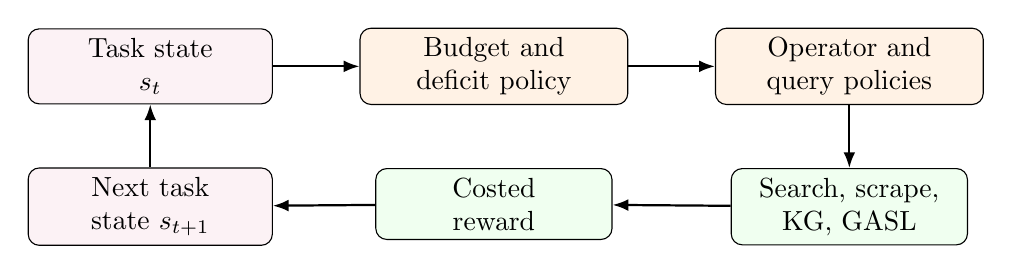
\begin{tikzpicture}[
  node distance=8mm and 11mm,
  box/.style={draw, rounded corners, align=center, minimum width=31mm,
    minimum height=9mm, fill=purple!5},
  policy/.style={draw, rounded corners, align=center, minimum width=34mm,
    minimum height=9mm, fill=orange!10},
  obs/.style={draw, rounded corners, align=center, minimum width=30mm,
    minimum height=9mm, fill=green!6},
  arr/.style={-{Latex[length=2mm]}, thick}
]
\node[box] (state) {Task state\\$s_t$};
\node[policy, right=of state] (top) {Budget and\\deficit policy};
\node[policy, right=of top] (sub) {Operator and\\query policies};
\node[obs, below=of sub] (obs) {Search, scrape,\\KG, GASL};
\node[obs, below=of top] (reward) {Costed\\reward};
\node[box, below=of state] (next) {Next task\\state $s_{t+1}$};

\draw[arr] (state) -- (top);
\draw[arr] (top) -- (sub);
\draw[arr] (sub) -- (obs);
\draw[arr] (obs) -- (reward);
\draw[arr] (reward) -- (next);
\draw[arr] (next) -- (state);
\end{tikzpicture}
\caption{Future hierarchical policy.  Existing operators remain available, but
their selection is scored against expected delayed reward.}
\label{fig:policy}
\end{figure}

\subsection{Policy surfaces}

The first learned policies should be narrow rerankers wrapped around existing
actions, not unconstrained generators.

\begin{longtable}{@{}p{0.18\linewidth}p{0.24\linewidth}p{0.22\linewidth}p{0.26\linewidth}@{}}
\caption{Decision surfaces for policy learning.}
\label{tab:policies}\\
\toprule
Surface & Current action & Learned replacement & Primary reward \\
\midrule
\endfirsthead
\toprule
Surface & Current action & Learned replacement & Primary reward \\
\midrule
\endhead
\bottomrule
\endfoot
Catalog frontier &
Prompt proposes broad search tasks. &
Rank source-family probes and expected answer-universe information gain. &
Closed completion bins per Firecrawl and LLM cost. \\
\addlinespace
Target deficit &
Static operator order plus LLM query construction. &
Rank deficit, operator, and query candidates jointly. &
New deduplicated row identities and required slots per cost. \\
\addlinespace
Source relevance &
Prompt judge accepts or rejects candidate hits. &
Calibrated gate that predicts delayed table reward and duplicate risk. &
Accepted sources that yield graph and table delta. \\
\addlinespace
Graph scope &
Source-neighborhood graph construction. &
Rank source neighborhoods and path scopes before GASL. &
GASL row yield, provenance quality, and extraction cost. \\
\addlinespace
Best-guess sidecars &
Fixed operator cascade. &
Contextual bandit over row-slot families and operators. &
Accepted sidecar slots per token and second. \\
\addlinespace
Stop/continue &
Completion state plus critique. &
Risk-sensitive stop policy constrained by open bins. &
Completeness reward minus over-search cost. \\
\end{longtable}

\subsection{Reward}

The existing table reward should become a costed task reward:

\[
R_t =
R_{\text{rows}} +
R_{\text{slots}} +
R_{\text{sources}} +
R_{\text{sidecars}} +
R_{\text{scope}}
- C_{\text{search}}
- C_{\text{scrape}}
- C_{\text{llm}}
- P_{\text{duplicate}}
- P_{\text{stale}}
\]

The major addition is \(R_{\text{scope}}\), a term that rewards closing
declared completion bins and establishing lower bounds.  Without it, a policy
can overfit to dense but narrow sources and ignore the task-level proof of
completeness.  Costs should be attached to the action that caused them:
Firecrawl search calls to query actions, scrape calls to candidate acceptance,
tokens to LLM actions, and wall time to all blocking actions.

\subsection{Offline before online}

The rollout path should be conservative:

\begin{enumerate}
  \item Instrument the static policy and store trajectories without changing
  behavior.
  \item Build offline action/outcome joins over prior \code{question_runs}.
  \item Generate deterministic preference pairs from observed reward:
  accepted high-yield action beats same-state zero-yield action; duplicate
  action loses to nonduplicate accepted action; no-cost deterministic sidecar
  action beats equal-yield LLM action.
  \item Add LLM preference labels only for ambiguous comparisons where delayed
  reward is close or confounded.
  \item Train a reranker or contextual-bandit head for one low-risk surface,
  starting with best-guess operator order or source relevance.
  \item Run off-policy evaluation and replay against held-out traces.
  \item Enable online use behind \code{--policy learned --policy-path ...} with
  small exploration and strict budget caps.
\end{enumerate}

\section{Required Code Changes}

\subsection{Trajectory events}

Add \code{question_pipeline/trajectory.py} with small immutable records:

\begin{verbatim}
DecisionPoint:
  decision_id
  run_id
  round_index
  surface
  state_ref
  candidate_actions
  selected_action_id
  policy_name
  policy_score

ActionRecord:
  action_id
  decision_id
  action_type
  target_id
  operator
  query
  expected_cost

ObservationRecord:
  observation_id
  action_id
  search_task_id
  source_id
  search_hits
  accepted
  skipped_reasons
  graph_delta
  table_delta
  best_guess_delta
  cost

RewardRecord:
  reward_id
  round_index
  action_ids
  component_scores
  total_reward
\end{verbatim}

Each record should be JSON-serializable and written to
\code{answers/trajectory.jsonl}.  The schema must be generic: no domain words,
no disease-specific slots, and no query-specific routing.

\subsection{Policy interface}

Add \code{question_pipeline/policy.py}:

\begin{verbatim}
class Policy(Protocol):
    def propose(
        self,
        surface: str,
        state: Mapping[str, Any],
        actions: Sequence[Mapping[str, Any]],
    ) -> PolicyDecision:
        ...
\end{verbatim}

The first implementation, \code{StaticTableFillPolicy}, should call the current
helpers:

\begin{itemize}
  \item \code{plan_catalog_operator()} for catalog searches;
  \item \code{plan_target_operator()} for target deficits;
  \item the existing fixed best-guess operator order;
  \item the current completion actionability check for stopping.
\end{itemize}

That wrapper gives the static system the same event stream as a future learned
policy.  CLI flags can then select a policy without changing pipeline code:

\begin{verbatim}
--policy static
--policy replay
--policy learned
--policy-path /path/to/model
--exploration-rate 0.02
\end{verbatim}

\subsection{Instrumentation points}

The recorder should be called where the code already chooses work:

\begin{longtable}{@{}p{0.30\linewidth}p{0.60\linewidth}@{}}
\caption{Minimal instrumentation plan.}
\label{tab:instrumentation}\\
\toprule
Code path & Event to record \\
\midrule
\endfirsthead
\toprule
Code path & Event to record \\
\midrule
\endhead
\bottomrule
\endfoot
\code{_enqueue_catalog_searches()} &
Catalog decision, all candidate catalog tasks, selected tasks, operator
metadata. \\
\code{_enqueue_target_deficit_searches()} &
Deficit decision, operator plan, candidate queries, rejected alternatives,
selected search tasks. \\
\code{SearchHarvester._accept_result_async()} &
Candidate source observation, scrape cost, relevance decision, accepted or
rejected URL, duplicate status. \\
\code{_ingest_papers()} &
Source-to-graph delta and extractor errors. \\
\code{_gasl_graph_for_round()} and \code{_run_gasl()} &
Graph-scope action, scoped node and edge counts, GASL result, repair counts,
produced artifacts. \\
\code{_run_best_guess_recovery()} &
Sidecar slot plan, operator order, per-operator candidates, accepted slots,
LLM token cost. \\
\code{_write_reward_exports()} &
Reward components linked to search task IDs, source IDs, and best-guess task
IDs. \\
\code{_record_task_goal()} &
Completion estimate, critique outcome, open bins, suggested queries, stop or
continue decision. \\
\end{longtable}

\subsection{Candidate actions, not only selected actions}

Learning from a trace requires knowing which alternatives were considered.
Current helpers usually return only the final query or task.  They should be
split into two phases:

\begin{enumerate}
  \item generate a small list of valid candidates under the current operator;
  \item let the policy rank candidates and select the subset to enqueue.
\end{enumerate}

The same split is useful for best-guess sidecars: build a queue of row-slot
families and legal operators, then let a policy spend the batch budget on the
highest expected marginal yield.

\subsection{Cost accounting}

Reward and trajectories need comparable costs across action types.  Add these
fields to search, source, GASL, and best-guess observations:

\begin{itemize}
  \item provider call count;
  \item provider credit estimate when available;
  \item returned hit count;
  \item fetched byte count;
  \item LLM model, prompt tokens, completion tokens, and retry count;
  \item wall-clock milliseconds;
  \item timeout or parse-error class.
\end{itemize}

The immediate use is analysis.  The future use is a reward penalty that can
prefer two high-yield LLM calls over twenty broad searches that produce only
duplicates.

\subsection{Offline builders}

Add read-only tools for offline learning:

\begin{itemize}
  \item \code{tools/build_table_fill_trajectories.py}: scan existing
  \code{question_runs}, join search outcomes, GASL states, table exports,
  best-guess artifacts, completion records, and reward snapshots into
  trajectories.
  \item \code{tools/score_table_fill_trajectories.py}: recompute reward under a
  chosen reward version.
  \item \code{tools/evaluate_table_fill_policy.py}: replay a policy over
  logged candidate sets and report off-policy acceptance, expected reward,
  duplicate rate, and unresolved completion bins.
\end{itemize}

\section{Preference Data for Multi-Turn Learning}

The first training data can come from the traces that already exist.
Useful deterministic preferences include:

\begin{itemize}
  \item A search action that accepted a source and later produced table rows is
  preferred to a same-deficit action that produced zero hits.
  \item A search action that only returned duplicate URLs is worse than one
  that found a new accepted source at similar cost.
  \item A source relevance decision is correct when the accepted source later
  produces graph and table delta; it is suspect when it produces no graph
  delta and no reusable completion evidence.
  \item A best-guess operator with positive marginal non-overlapping slots is
  preferred to an operator with repeated zero yield for the same slot family.
  \item A completion action that closes a defensible row-family lower bound is
  preferred to one that merely reiterates an already-open issue.
\end{itemize}

These preferences should be scoped by state.  A cheap same-row scan with zero
yield in one table should not globally ban same-row scans; it only says the
operator was weak for that observed row-slot distribution.

\section{Evaluation Plan}

\subsection{Holdout tasks}

Evaluation needs multiple query trees with different table structures.  The
learned policy should be trained on some tasks and replayed on held-out tasks.
Holdouts should include:

\begin{itemize}
  \item source-level numeric aggregation from papers;
  \item source-level rows that require supplementary tables;
  \item time-series or subnational rows where row cardinality can explode;
  \item best-guess-heavy tables where location or date must be inferred from
  source context;
  \item tasks where catalog probing should happen before target filling.
\end{itemize}

\subsection{Metrics}

Report both immediate and delayed metrics:

\begin{itemize}
  \item accepted sources per search call;
  \item new deduplicated row identities per accepted source;
  \item required slot fill rate;
  \item best-guess slot precision and marginal yield;
  \item cost per marginal source-backed row;
  \item duplicate URL rate;
  \item blocked or timeout rate;
  \item number of open critical completion bins;
  \item final completion acceptance rate under the critic.
\end{itemize}

The final metric should never be just row count.  A dense but narrow table can
increase reward while failing the task because it leaves the answer universe
unbounded.

\section{Implementation Roadmap}

\begin{enumerate}
  \item \textbf{Trajectory-only instrumentation.}  Add recorder calls while
  keeping \code{--policy static} as the only active policy.  Verify that
  re-running a table-fill task produces identical search tasks and tables.
  \item \textbf{Offline trajectory builder.}  Backfill older round folders into
  the same schema so analysis can start before new runs accumulate.
  \item \textbf{Costed reward v2.}  Add provider and wall-time costs, plus
  completion-bin closure reward.
  \item \textbf{Candidate preservation.}  Change catalog, target, and
  best-guess planners to store candidate actions before selection.
  \item \textbf{Source relevance calibration.}  Train and replay a gate
  reranker because source acceptance is narrow, frequent, and already has a
  clear delayed label.
  \item \textbf{Best-guess operator bandit.}  Learn sidecar operator ordering
  from per-slot marginal yields.
  \item \textbf{Search operator reranker.}  Learn a reranker over generic
  operator and query candidates for catalog and target deficits.
  \item \textbf{Top-level budget policy.}  Learn when to spend on completion
  probes, target searches, ingestion, GASL, and best-guess recovery.
  \item \textbf{Online canary.}  Enable learned ranking only for a small
  fraction of candidates under budget caps, log all counterfactual candidate
  scores, and keep the static policy as the fallback.
\end{enumerate}

\section{Conclusion}

The current table-fill system is already a stateful iterative aggregator.  It
records enough evidence to show successful adaptation, as in the round-28
context pivot, and enough evidence to expose weak adaptation, as in the
round-29 and round-30 low-yield pivots.  The missing layer is not another
question-specific search prompt.  It is a generic trajectory and policy layer
that turns those observed outcomes into reusable training examples.

The fastest path is to make the static controller observable first.  Once every
catalog action, target action, source-gate decision, graph-scope choice, GASL
attempt, best-guess operator, cost, and delayed reward has a stable ID, the
same run logs can support deterministic preferences, offline replay, and then
cautious online policy learning.

\appendix

\section{Trajectory Join Keys}

\begin{longtable}{@{}p{0.22\linewidth}p{0.68\linewidth}@{}}
\toprule
Key & Purpose \\
\midrule
\endfirsthead
\toprule
Key & Purpose \\
\midrule
\endhead
\bottomrule
\endfoot
\code{run_id} &
Groups every outer round and generated artifact for one table-fill invocation. \\
\code{round_index} &
Identifies the outer loop iteration.  This is not a search wave or
best-guess batch. \\
\code{decision_id} &
Links a policy state to the action candidates it ranked. \\
\code{action_id} &
Links a selected action to search, source, GASL, or best-guess observations. \\
\code{search_task_id} &
Links query construction to Firecrawl hits, duplicate URLs, relevance
judgments, and accepted sources. \\
\code{source_id} &
Links an accepted source to graph records, GASL tables, and provenance-bearing
rows. \\
\code{best_guess_task_id} &
Links a missing row slot to deterministic or LLM sidecar candidates. \\
\code{table_spec_id} &
Separates runs that work on different carried-forward table definitions. \\
\end{longtable}

\section{Design Constraints}

\begin{itemize}
  \item The policy API must be generic over question and table schema.
  \item Operators may encode search tactics but not domain vocabulary.
  \item Learned policies must choose among legal planner actions; they should
  not bypass completion, provenance, or source-relevance constraints.
  \item A run must remain reproducible with \code{--policy static}.
  \item Online exploration must be budget capped and must log rejected
  alternatives.
  \item Reward versions must be explicit so old trajectories can be rescored.
\end{itemize}

\end{document}
